% This is a simple template for a LaTeX document using the "article" class.
% See "book", "report", "letter" for other types of document.

\documentclass[10pt]{article} % use larger type; default would be 10pt

\usepackage[utf8]{inputenc} % set input encoding (not needed with XeLaTeX)

%%% Examples of Article customizations
% These packages are optional, depending whether you want the features they provide.
% See the LaTeX Companion or other references for full information.

%%% PAGE DIMENSIONS
\usepackage{geometry} % to change the page dimensions
\geometry{a4paper} % or letterpaper (US) or a5paper or....
\usepackage{setspace}
\usepackage{parskip}
\parskip = 0.3 \baselineskip %\advance\parskip by 0pt plus 2pt% to change between paragraphs space
% \geometry{margin=2in} % for example, change the margins to 2 inches all round
% \geometry{landscape} % set up the page for landscape
%   read geometry.pdf for detailed page layout information

% \usepackage{gravarphicx} % support the \includegravarphics command and options
% \usepackage[parfill]{parskip} % Activate to begin paragraphs with an empty line rather than an indent

%%% PACKAGES
\usepackage{{booktabs}} % for much better looking tables
\usepackage{array} % for better arrays (eg matrices) in maths
\usepackage{paralist} % very flexible & customisable lists (eg. enumerate/itemize, etc.)
\usepackage{verbatim} % adds environment for commenting out blocks of text & for better verbatim
\usepackage{subfigure} % make it possible to include more than one captioned figure/table in a single float
% These packages are all incorporated in the memoir class to one degree or another...
\usepackage[fleqn]{amsmath}
\usepackage{amssymb}
\usepackage{enumitem}
\usepackage{amsthm}
\usepackage{graphicx}
\usepackage{filecontents}
\usepackage{natbib}
\usepackage{blindtext}
\usepackage{titlesec}
\usepackage[table,xcdraw]{xcolor}
\usepackage{{multirow}}


%%% HEADERS & FOOTERS
\usepackage{fancyhdr} % This should be set AFTER setting up the page geometry
\pagestyle{plain} % options: empty , plain , fancy
\renewcommand{\headrulewidth}{0pt} % customise the layout...
\lhead{}\chead{}\rhead{}
\lfoot{}\cfoot{\thepage}\rfoot{}

%%% SECTION TITLE APPEARANCE
\usepackage{sectsty}
\allsectionsfont{\rmfamily\bfseries\upshape} % (See the fntguide.pdf for font help)
% (This matches ConTeXt defaults)

%%% ToC (table of contents) APPEARANCE
\usepackage[nottoc,notlof,notlot]{tocbibind} % Put the bibliography in the ToC
\usepackage[titles,subfigure]{tocloft} % Alter the style of the Table of Contents
\renewcommand{\cftsecfont}{\rmfamily\mdseries\upshape}
\renewcommand{\cftsecpagefont}{\rmfamily\mdseries\upshape} % No bold!

\usepackage[colorlinks,citecolor=black,urlcolor=black,bookmarks=false,hypertexnames=true]{hyperref} 

%%% END Article customizations



%%% The "real" document content comes below...

\title{MECON6102 Problem Set 2}
\author{Xing Mingjie}
\date{\today} % Activate to display a given date or no date (if empty),
         % otherwise the current date is printed 

\begin{document}
\maketitle

% \tableofcontents



\section{Data}
    \subsection{Description}
    \begin{table}[centering]
\caption{Data Description}
\label{tab:data_description}
\begin{tabular}{lrrrrr}
\toprule
 & count & mean & std & min & max \\
\midrule
\textbf{default\_label} & 13982.00 & 0.02 & 0.15 & 0.00 & 1.00 \\
\textbf{age} & 13982.00 & 41.66 & 14.56 & 17.00 & 66.00 \\
\textbf{gender} & 13982.00 & 0.46 & 0.50 & 0.00 & 1.00 \\
\textbf{edu} & 13982.00 & 1.69 & 1.10 & 0.00 & 4.00 \\
\textbf{housing} & 13982.00 & 0.63 & 0.48 & 0.00 & 1.00 \\
\textbf{income} & 13982.00 & 7426.48 & 6226.68 & 650.42 & 37515.37 \\
\textbf{job\_occupation} & 13982.00 & 0.34 & 0.56 & 0.00 & 2.00 \\
\textbf{past\_bad\_credit} & 13982.00 & 0.96 & 0.19 & 0.00 & 1.00 \\
\textbf{married} & 13982.00 & 0.53 & 0.50 & 0.00 & 1.00 \\
\bottomrule
\end{tabular}
\end{table}


    Table \ref{tab:data_description} shows the summary statistics of the data. The data set contains 13982 observations and 9 variables. The dependent variable is the default label, which is a binary variable indicating whether the individual defaults. 

    \begin{figure}
        \centering
        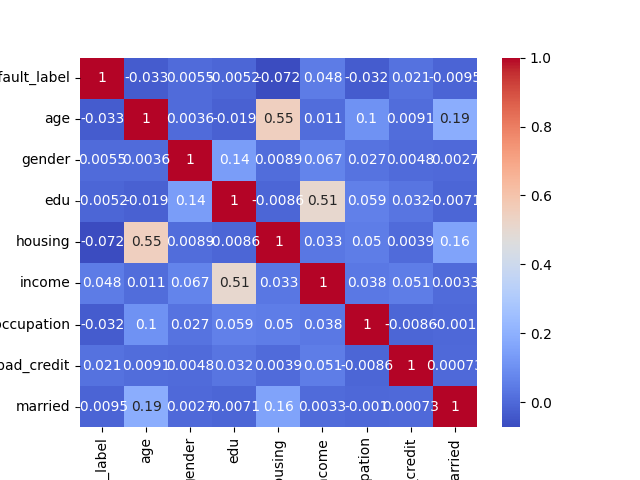
\includegraphics[width=0.8\textwidth]{"../fig/variable_heatmap.png"}
        \caption{Heat map of the correlation matrix of the variables}
        \label{fig:variable_heatmap}
    \end{figure}
    Figure \ref{fig:variable_heatmap} shows the heat map of the correlation matrix of the features and target. Most of the features are arguably uncorrelated. There is a high correlation between housing and age at 0.55. The correlation between income and education level is 0.51, which captures the wage premium of education.
    \subsection{Data Preprocessing}
    \begin{figure}
        \centering
        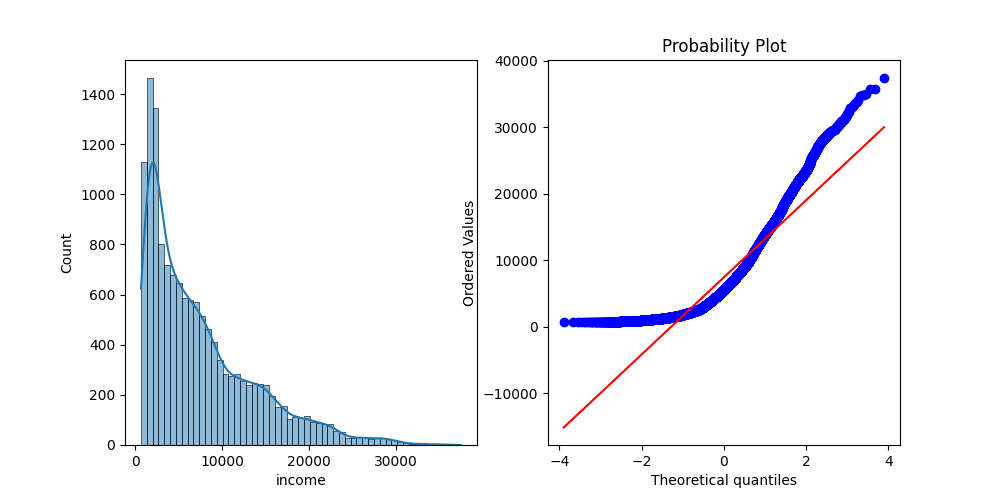
\includegraphics[width=0.8\textwidth]{"../fig/income_distribution.png"}
        \caption{Income Distribution}
        \label{fig:income_skew}
    \end{figure}
    Figure \ref{fig:income_skew} shows the distribution and the skewness of feature \texttt{income}. The distribution is right-skewed. The report uses the log transformation to reduce the skewness of the feature for better performance in models.
    \begin{figure}
        \centering
        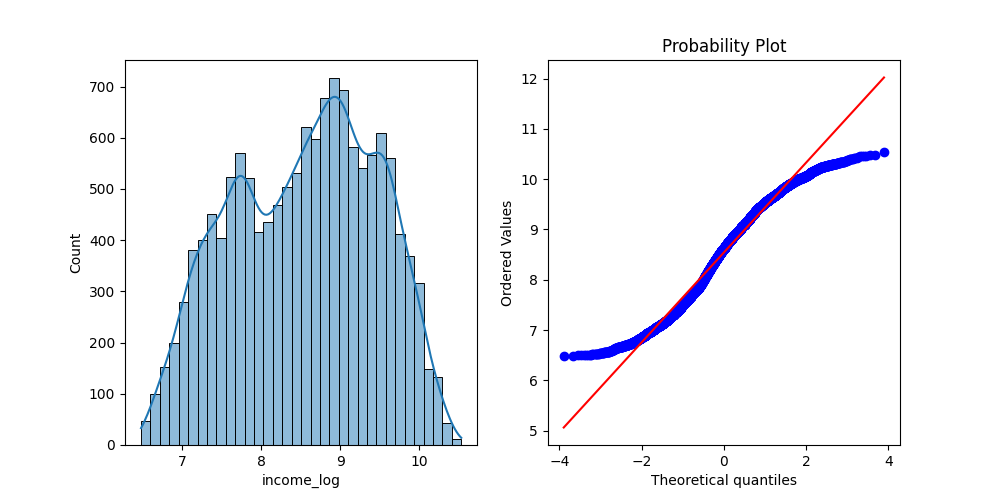
\includegraphics[width=0.8\textwidth]{"../fig/income_distribution_log_transform.png"}
        \caption{Income Distribution After Log Transformation}
        \label{fig:income_log}
    \end{figure}

    Figure \ref{fig:income_log} shows the distribution of the feature \texttt{income} after the log transformation. The distribution is more symmetric after the transformation and helps boost model performance in our exercise.

\section{Model Comparison}
    \subsection{Simple Logistic Model}
    \begin{figure}
        \centering
        \subfigure[Panel A]{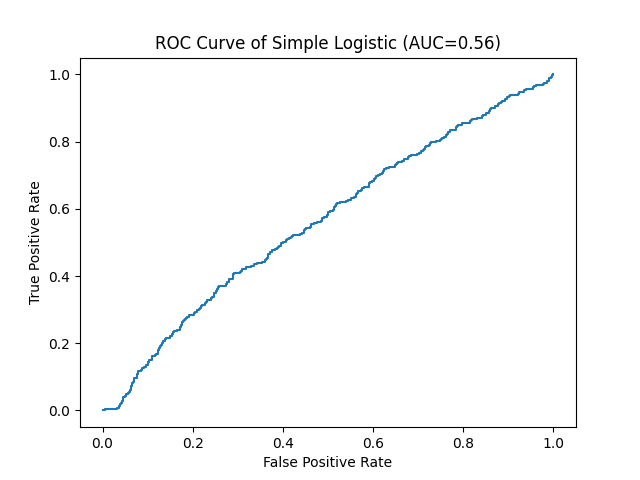
\includegraphics[width=0.4\textwidth]{"../fig/roc_curve_Simple Logistic.png"}}
        \hfill
        \subfigure[Panel B]{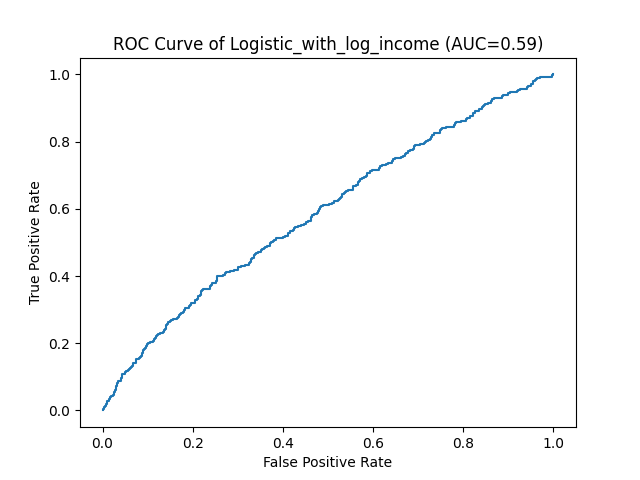
\includegraphics[width=0.4\textwidth]{"../fig/roc_curve_Logistic_with_log_income.png"}}
        \caption{ROC Curve of Simple Logistic Model}
        \label{fig:roc_simlogistic}
    \end{figure}

    Panel A of figure \ref{fig:roc_simlogistic} shows the ROC curve of the simple logistic regression model with feature \texttt{past\_bad\_credit} and \texttt{income} and the Panel B is the simple model with log-transformed \texttt{income}. The AUC is 0.56 for simple model, and 0.59 for simple logistic with log-transformed income. The predictive power is close to a random draw, but the log transformation add to the performance of model. In the rest of the exercise, we use the log-transformed income instead of the original income.

    \subsection{Full Logistic Model}

    \begin{figure}
        \centering
        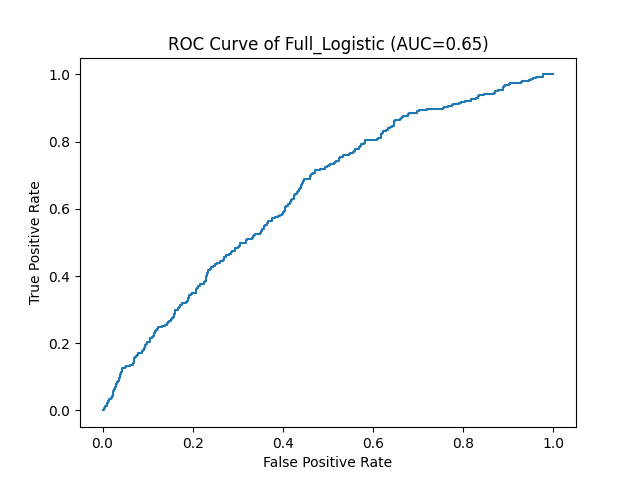
\includegraphics[width=0.8\textwidth]{"../fig/roc_curve_Full_Logistic.png"}
        \caption{ROC Curve of Full Logistic Regression}
        \label{fig:roc_fulllogistic}
    \end{figure}
    In a full logistic model with log-transformed income in Figure \ref{fig:roc_fulllogistic}, we have an AUC of 0.69, which is a significant improvement over the simple model. The full model includes all the features in the data set. 
    
    \subsection{non-linear models}
    \begin{figure}
        \centering
        \subfigure{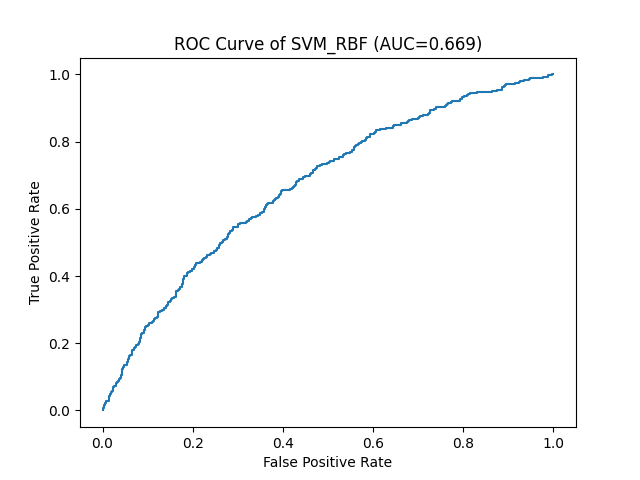
\includegraphics[width=0.3\textwidth]{"../fig/roc_curve_SVM_RBF.png"}}
        \hfill
        \subfigure{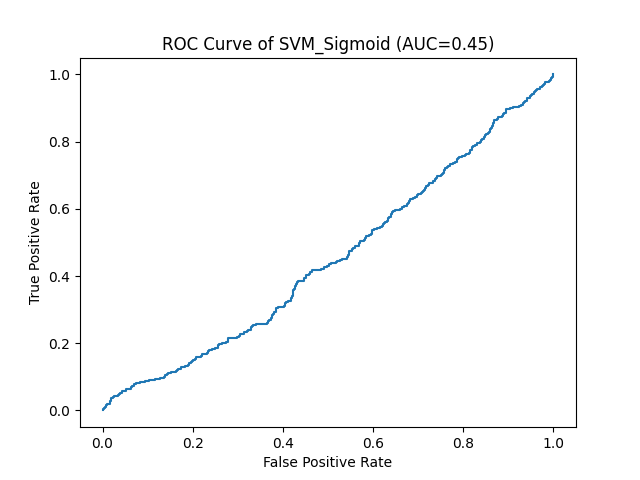
\includegraphics[width=0.3\textwidth]{"../fig/roc_curve_SVM_Sigmoid.png"}}
        \hfill
        \subfigure{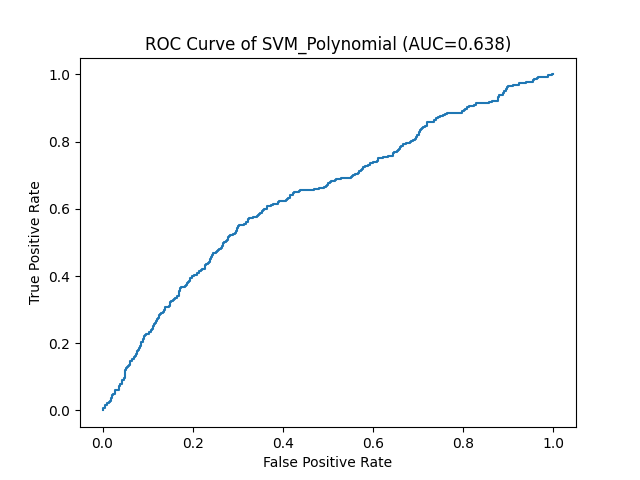
\includegraphics[width=0.3\textwidth]{"../fig/roc_curve_SVM_Polynomial.png"}}
        \caption{SVM with RBF, sigmoid, polynomial kernel}
        \label{fig:three_svm}
    \end{figure}

    This part reports the non-linear models.
    The SVM model with RBF as kernel has an AUC of 0.67, with sigmoid 0.45, with polynomial 0.64, as reported in Figure \ref{fig:three_svm}. The RBF kernel has the best performance among the three kernels. Sigmoid performs even worse than random classification. In the rest of the exercise, we use the RBF kernel for SVM.

    In the literature, \cite{Bazzanaetal2023} and \cite{Wu2022} proposes Neural Network, XGBoosting and Random Forest as the best predictive algorithms for default risk, with AUC around 0.97.

    \subsection{Within-Sample Performance}
    \begin{table}
\caption{AUC Comparison}
\label{tab:auc_compare}
\begin{tabular}{lr}
\toprule
Model & auc \\
\midrule
Simple Logistic & 0.563 \\
Simple Logistic with log income & 0.589 \\
Full Logistic & 0.685 \\
SVM RBF & 0.669 \\
SVM Sigmoid & 0.547 \\
SVM Poly & 0.638 \\
Random Forest & 1.000 \\
XGBoosting & 0.980 \\
Neural Network & 0.720 \\
\bottomrule
\end{tabular}
\end{table}

    Table \ref{tab:auc_compare} reports the with-in sample of each model as we discussed above. The two best performers are Random Forest and XGBoosting, with AUC of 1 and 0.98, showing an overfitting problem. The rest part of the report focuses on hypertuning models to improve the out-of-sample performance. 

    \subsection{Out-of-Sample Performance}
    \begin{table}
\caption{AUC Comparison (Out of Sample)}
\label{tab:auc_oos_compare}
\begin{tabular}{lr}
\toprule
Model & auc \\
\midrule
Logistic & 0.69 \\
SVM RBF & 0.52 \\
Random Forest & 0.58 \\
XGBoosting & 0.57 \\
Neural Network & 0.61 \\
\bottomrule
\end{tabular}
\end{table}

    Table \ref{tab:auc_oos_compare} reports the baseline (default parameter suggested by the package) out-of-sample performance of each model in the \texttt{auc} column. The full logistic model has the best performance with an AUC of 0.686. The SVM model with RBF kernel has a lowest AUC of 0.518. 

    \subsubsection{Hypertuning}
    The baseline, hypertuned parameters, and best parameters are reported in the jupyter notebook. We leverage \texttt{GridSearchCV} to hypertune the models to maximize out-of-sample roc-auc performance. We provide a dictionary of hyperparameters to each model and do cross validation of 5-fold. As we can see from the \texttt{auc\_tuned} column of table \ref{tab:auc_oos_compare}, after hypertuning there is generally a 10\% increase in the performance of each model. The best performer is still the Logistic model, though with only marginal improvement.
    


\newpage
\footnotesize
\bibliographystyle{apalike}
\bibliography{ref}

\end{document}